\begin{frame}
  \frametitle{Booting with U-Boot}
  \begin{itemize}
  \item On ARM32, U-Boot can boot \code{zImage} (\code{bootz} command)
  \item On ARM64 or RISC-V, it boots the \code{Image} file (\code{booti} command)
  \item In addition to the kernel image, U-Boot should also pass a
        DTB to the kernel.
  \item The typical boot process is therefore:
    \begin{enumerate}
    \item Load \code{zImage} at address X in memory
    \item Load \code{<board>.dtb} at address Y in memory
    \item Start the kernel with \code{boot[z|i] X - Y} \\
      The \code{-} in the middle indicates no {\em initramfs}
    \end{enumerate}
  \end{itemize}
\end{frame}

\begin{frame}
  \frametitle{Kernel command line}
  \begin{itemize}
  \item In addition to the compile time configuration, the kernel
    behavior can be adjusted with no recompilation using the {\bf
      kernel command line}
  \item The kernel command line is a string that defines various
    arguments to the kernel
    \begin{itemize}
    \item It is very important for system configuration
    \item \code{root=} for the root filesystem (covered later)
    \item \code{console=} for the destination of kernel messages
    \item Example: \code{console=ttyS0 root=/dev/mmcblk0p2 rootwait}
    \item Many more exist. The most important ones are documented
          in \kdochtml{admin-guide/kernel-parameters} in kernel
          documentation.
    \end{itemize}
  \end{itemize}
\end{frame}

\begin{frame}
  \frametitle{Passing the kernel command line}
  \begin{columns}
    \column{0.7\textwidth}
    \begin{itemize}
    \item U-Boot carries the Linux kernel command line string in its
      \code{bootargs} environment variable
    \item Right before starting the kernel, it will store the contents of
      \code{bootargs} in the \code{chosen} section of the Device Tree
    \item The kernel will behave differently depending on its
      configuration:
      \begin{itemize}
      \item If \kconfig{CONFIG_CMDLINE_FROM_BOOTLOADER} is set:\\
        The kernel will use only the string from the bootloader
      \item If \kconfig{CONFIG_CMDLINE_FORCE} is set:\\
        The kernel will only use the string received at configuration
        time in \kconfig{CONFIG_CMDLINE}
      \item If \kconfig{CONFIG_CMDLINE_EXTEND} is set:\\
        The kernel will concatenate both strings
      \end{itemize}
    \end{itemize}
    \column{0.3\textwidth}
    \tiny See the "Understanding U-Boot Falcon Mode"
    presentation from Michael Opdenacker, for details about how U-Boot
    boots Linux.\\
    \vspace{0.6cm}
    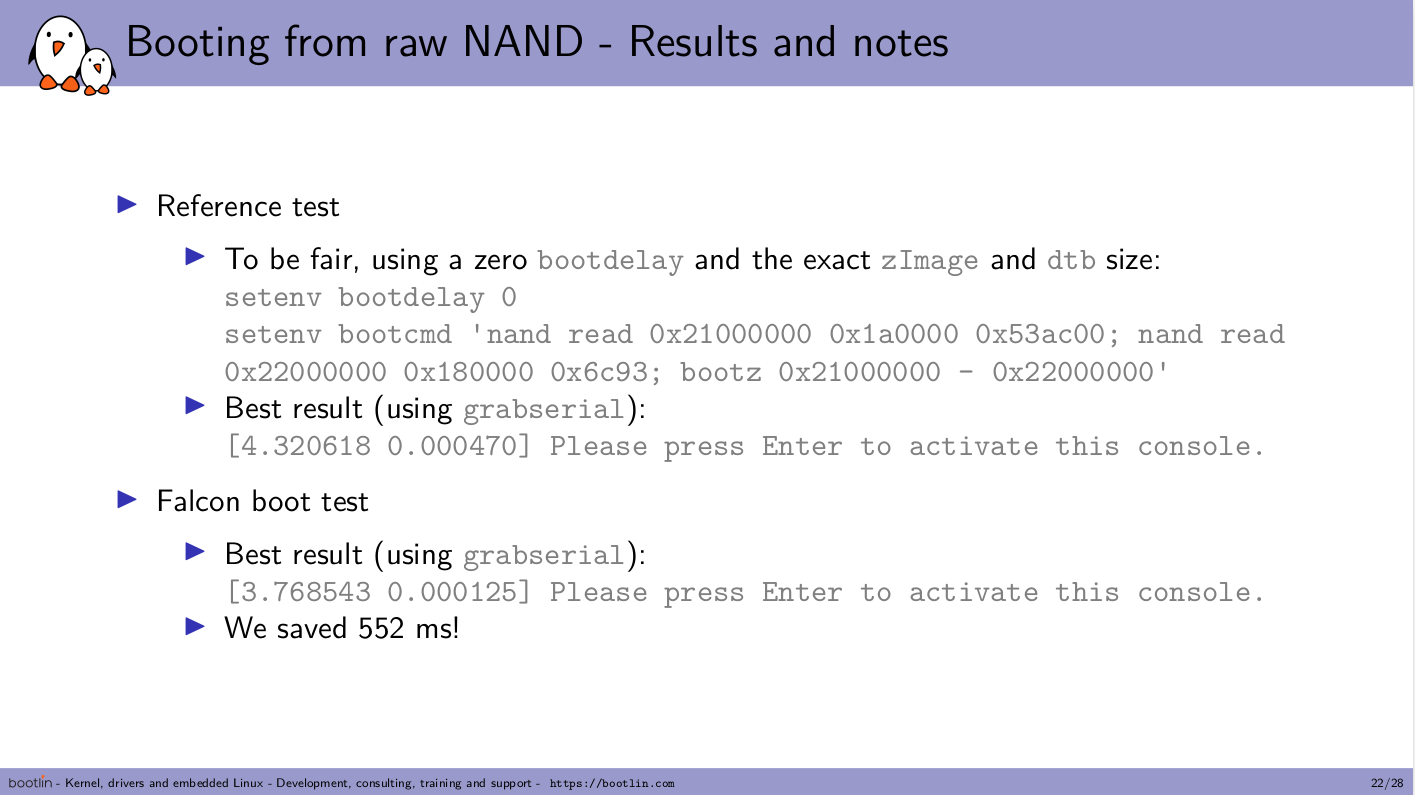
\includegraphics[width=\textwidth]{slides/sysdev-kernel-booting/understanding-falcon-mode-presentation.png}\\
    \vspace{0.4cm}
    \tiny Slides: \url{https://bootlin.com/pub/conferences/2021/lee/}\\
    Video: \url{https://www.youtube.com/watch?v=LFe3x2QMhSo}
  \end{columns}
\end{frame}

\begin{frame}
  \frametitle{Kernel log}
  \begin{itemize}
  \item The kernel keeps its messages in a circular buffer in memory
    \begin{itemize}
    \item The size is configurable using \kconfig{CONFIG_LOG_BUF_SHIFT}
    \end{itemize}
  \item When a module is loaded, related information is available in the
    kernel log.
  \item Kernel log messages are available through the \code{dmesg}
    command ({\bf d}iagnostic {\bf mes}sa{\bf g}e)
  \item Kernel log messages are also displayed on the console pointed by
    the \code{console=} kernel command line argument
    \begin{itemize}
    \item Console messages can be filtered by level using the
      \code{loglevel} parameter
    \item Example: \code{console=ttyS0 loglevel=5}
    \end{itemize}
  \item It is possible to write to the kernel log from user space:
  \code{echo "<n>Debug info" > /dev/kmsg}
  \end{itemize}
\end{frame}
